\documentclass[border=1pt, 12pt, tikz]{standalone}

\newcommand\wideOne{2cm}%{3cm}
\newcommand\wideTwo{3.5cm}%{4cm}
\newcommand\wideThree{1.5cm}
\newcommand\wideFour{2cm}
\newcommand\distOne{2cm}
\newcommand\distTwo{1cm}

\begin{document}
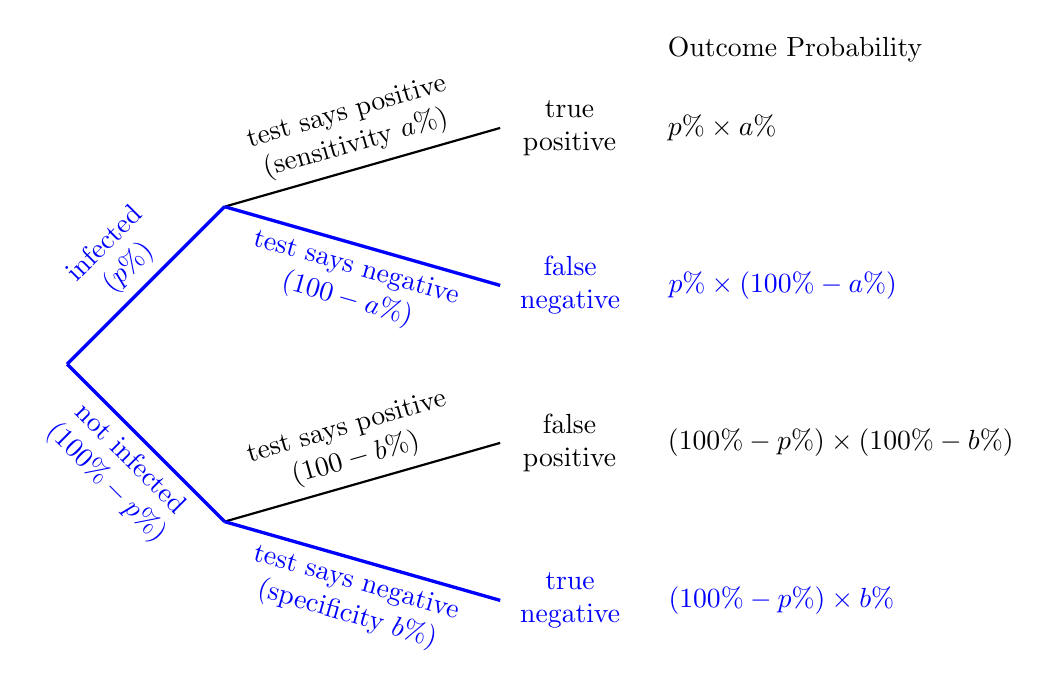
\begin{tikzpicture}[scale=1]

% 1st level
\draw[very thick, blue]%
   (0,0) 
   -- node[above, sloped, align=center]
      {infected\\$(p\%)$}
   (\wideOne,\distOne);
\draw[very thick, blue] 
   (0,0) 
   -- node[below, sloped, align=center]
      {not infected\\$(100\%-p\%)$} 
   (\wideOne,-\distOne);

% 2nd, 3rd and 4th Level
\draw[thick] 
   (\wideOne,\distOne)
   -- node[above, align=center, sloped]
      {test says positive\\(sensitivity $a\%$)}
   ++ (\wideTwo,\distTwo) 
      node[right, align=center, text width=\wideThree]
      {true\\positive}
   ++ (\wideFour,0) 
      node[right]
      {$p\%\times a\%$}
   ++ (0,1)
      node[right]
      {Outcome Probability}
   ; 
\draw[very thick, blue] 
   (\wideOne,\distOne) 
   -- node[below, align=center, sloped]
      {test says negative\\$(100-a\%)$}
   ++ (\wideTwo,-\distTwo) 
      node[right, align=center, text width=\wideThree]
      {false\\negative}
   ++ (\wideFour,0) 
      node[right]
      {$p\%\times (100\%-a\%)$}
   ;
\draw[thick] 
   (\wideOne,-\distOne) 
   -- node[above, align=center, sloped]
      {test says positive\\$(100-b\%)$}
   ++ (\wideTwo,\distTwo) 
      node[right, align=center, text width=\wideThree]
      {false\\positive}
   ++ (\wideFour,0) 
      node[right]
      {$(100\%-p\%)\times (100\%-b\%)$}
   ;  
\draw[very thick, blue] 
   (\wideOne,-\distOne)
   -- node[below, align=center, sloped]
      {test says negative\\(specificity $b\%$)}
   ++ (\wideTwo,-\distTwo) 
      node[right, align=center, text width=\wideThree]
      {true\\negative}
   ++ (\wideFour,0) 
      node[right]
      {$(100\%-p\%)\times b\%$}
   ; 
\end{tikzpicture}
\end{document}


% \newcommand\wideOne{3cm}
% \newcommand\wideTwo{3.5cm}
% \newcommand\wideThree{2.7cm}
% \newcommand\wideFour{3cm}
% \newcommand\distOne{2cm}
% \newcommand\distTwo{1cm}

% \begin{document}
% \begin{tikzpicture}[scale=1]

% % 1st level
% \draw[thick]%
%    (0,0) 
%    -- node[above, sloped, align=center]
%       {1st is heart} 
%    (\wideOne,\distOne);
% \draw[thick] 
%    (0,0) 
%    -- node[below, sloped, align=center]
%       {1st is not heart} 
%    (\wideOne,-\distOne);

% % 2nd, 3rd and 4th Level
% \draw[thick] 
%    (\wideOne,\distOne)
%    -- node[above, align=center, sloped]
%       {2nd is heart}
%    ++ (\wideTwo,\distTwo) 
%       node[right, align=center, text width=\wideThree]
%       {1st is heart and\\2nd is heart}
%    ; 
% \draw[thick] 
%    (\wideOne,\distOne) 
%    -- node[below, align=center, sloped]
%       {2nd is not heart}
%    ++ (\wideTwo,-\distTwo) 
%       node[right, align=center, text width=\wideThree]
%       {1st is heart and 2nd not heart}
%    ;
% \draw[thick] 
%    (\wideOne,-\distOne) 
%    -- node[above, align=center, sloped]
%       {2nd is heart}
%    ++ (\wideTwo,\distTwo) 
%       node[right, align=center, text width=\wideThree]
%       {1st not heart and 2nd heart}
%    ;  
% \draw[thick] 
%    (\wideOne,-\distOne)
%    -- node[below, align=center, sloped]
%       {2nd is not heart}
%    ++ (\wideTwo,-\distTwo) 
%       node[right, align=center, text width=\wideThree]
%       {1st not heart and 2nd not heart}
%    ; 
% \end{tikzpicture}
% \end{document}
